%The ``size'' of the speckles is a function of the wavelength of the light,
%the size of the laser beam which illuminates the first surface, and the
%distance between this surface and the surface where the speckle pattern is
%formed. This is the case because when the angle of scattering changes such
%that the relative path difference between light scattered from the centre
%of the illuminated area compared with light scattered from the edge of the
%illuminated changes by λ, the intensity becomes uncorrelated. Dainty [1]
%derives an expression for the mean speckle size as λz/L where L is the
%width of the illuminated area and z is the distance between the object and
%the location of the speckle pattern.

Following \name{Goodman} and \name{Dainty}, we define the size of a
speckle in terms of the area of the normalized
autocovariance function of the speckle intensity pattern, $c_I(\Delta x,
\Delta y)$.  The normalized autocovariance function is defined in terms of
the autocorrelation $\Gamma_I(\Delta x, \Delta y)$ by 
\begin{equation}
c_I(\Delta x, \Delta y) = \frac{\Gamma_I(\Delta x, \Delta y) - \bar{I}^2}{\bar{I}^2}
\end{equation}
and the autocorrelation is defined as
\begin{equation}
\Gamma_I(\Delta x, \Delta y) = \intinfty\intinfty I(x,y) \tilde{I}(x+\Delta x,y+\Delta y) \md x \md y
\end{equation}
For computation on real images, the integral is replaced by a sum.  Taking
advantage of the Wiener–Khinchin theorem, the autocorrelation is simply the
Fourier transform of the power spectral density, vis.
\begin{equation}
\Gamma_I(\Delta x, \Delta y) = \ff{|I(x,y)|^2}(\Delta x, \Delta y)
\end{equation}
and thus  $c_I(\Delta x, \Delta y)$ can be efficiently calculated on a
computer\footnote{For example in MATLAB this is implimented with
\texttt{xcov(I,'coeff')}}.

With these definitions out of the way, the area of $c_I(\Delta x, \Delta
y)$ is simply its integral over $\Delta x$ and $\Delta y$
\begin{align}
\mathscr{A}_c &= \intinfty\intinfty c_I(\Delta x, \Delta y) \md \Delta x \md \Delta y\\
&=\frac{(\lambda z)^2}{A}
\label{eqn:spotsize}
\end{align}

Conceptually, \Equation{eqn:spotsize} can be thought of as follows: the
difference between a ``bright'' spot and a ``dark'' spot in a speckle field
occurs when\ldots
\textit{This is the case because when the angle of scattering changes such
that the relative path difference between light scattered from the centre
of the illuminated area compared with light scattered from the edge of the
illuminated changes by lambda, the intensity becomes uncorrelated.}

We have measured the speckle size in the experiment and found that, in
apparent contradiction with \Equation{eqn:spotsize}, the speckle size does
\textit{not} change with spot size, at least for long range surface
plasmons.  This is evidenced in \Figure{fig:spotsize} for three different
spot sizes.  Here we have made a qualiatative measurement of the scattering
spot size by fitting a gaussian to its transverse dimension, and reporting
the full width at half maximum of that measurement as the spot size.

\begin{figure}[ht]
 \centering
 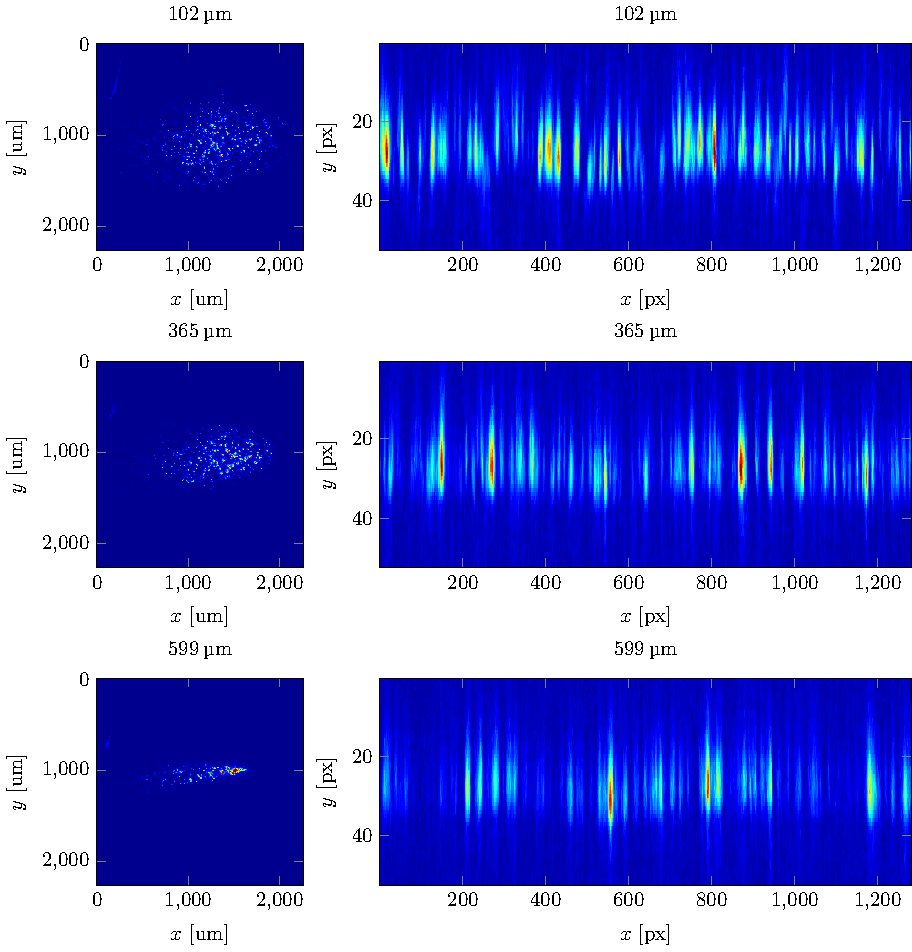
\includegraphics[keepaspectratio]{speckle/figures/spotsize/test.pdf}
 \caption{Speckle size versues spot size.  Inset images show an example of
 the raw spot size data from which the plot was computed.  Inset images are
 \SI{2.26x2.26}{\milli\meter} with major ticks at
 \SI{500}{\micro\meter} intervals.}
 \label{fig:spotsize}
\end{figure}
